\documentclass{sigchi}

% Load basic packages
\usepackage{balance}  % to better equalize the last page
\usepackage{graphics} % for EPS, load graphicx instead
\usepackage[T1]{fontenc}
\usepackage{txfonts}
\usepackage{mathptmx}
\usepackage[pdftex]{hyperref}
\usepackage{color}
\usepackage{booktabs}
\usepackage{textcomp}
% Some optional stuff you might like/need.
\usepackage{microtype} % Improved Tracking and Kerning
% \usepackage[all]{hypcap}  % Fixes bug in hyperref caption linking
\usepackage{ccicons}  % Cite your images correctly!
% \usepackage[utf8]{inputenc} % for a UTF8 editor only

% Paper metadata (use plain text, for PDF inclusion and later
% re-using, if desired).  Use \emtpyauthor when submitting for review
% so you remain anonymous.
\def\plaintitle{Measuring career preparedness with topic modeling}
\def\plainauthor{Michel Rouly}
\def\emptyauthor{}
\def\plainkeywords{employability; skills; topic modeling; natural language processing; machine learning
}
\def\plaingeneralterms{Topic Modeling}

% llt: Define a global style for URLs, rather that the default one
\makeatletter
\def\url@leostyle{%
  \@ifundefined{selectfont}{
    \def\UrlFont{\sf}
  }{
    \def\UrlFont{\small\bf\ttfamily}
  }}
\makeatother
\urlstyle{leo}

% To make various LaTeX processors do the right thing with page size.
\def\pprw{8.5in}
\def\pprh{11in}
\special{papersize=\pprw,\pprh}
\setlength{\paperwidth}{\pprw}
\setlength{\paperheight}{\pprh}
\setlength{\pdfpagewidth}{\pprw}
\setlength{\pdfpageheight}{\pprh}

% Make sure hyperref comes last of your loaded packages, to give it a
% fighting chance of not being over-written, since its job is to
% redefine many LaTeX commands.
\definecolor{linkColor}{RGB}{6,125,233}
\hypersetup{%
  pdftitle={\plaintitle},
  pdfauthor={\plainauthor},
% Use \emptyauthor for submission version.
%  pdfauthor={\emptyauthor},
  pdfkeywords={\plainkeywords},
  bookmarksnumbered,
  pdfstartview={FitH},
  colorlinks,
  citecolor=black,
  filecolor=black,
  linkcolor=black,
  urlcolor=linkColor,
  breaklinks=true,
}

\begin{document}

\title{\plaintitle}

\numberofauthors{1}

\author{%
  \alignauthor%
  Michel Rouly\\
  \affaddr{Georgia Institute of Technology}\\
  \email{jrouly3@gatech.edu}
}

\maketitle

\begin{abstract}
  Entry level workforce positions requiring a minimum of postsecondary education is becoming more and more prevalent.~\cite{carnevale2010}
  Degrees are being used as a semi standard basis for knowledge and skill expectations of new employees.
  Consequently increasingly many young people are turning to postsecondary education as a means of becoming qualified for a job.
  In turn, educational institutions must ensure that curricula are suited to the expectations of educators, recruiters, and students.
  Is it possible to determine whether postsecondary institutions are preparing students for the workforce?
  This paper introduces an application of ``Natural Language Processing'' (NLP) to large corpora of human language documents in an effort to measure this.
  The contribution is a method of retrieving, cleaning, and processing these documents to then measure the degree of overlap between educational outcomes and workforce expectations.
\end{abstract}


\category{K.4.m}{Computers and Society}{Miscellaneous}
\category{I.2.7}{Natural Language Processing}{Text analysis}

\keywords{\plainkeywords}

\section{Introduction}

More and more frequently, young Americans entering the workforce are encountering educational requirements for entry level positions.~\cite{carnevale2010}
This phenomenon may be viewed as a consequence of attempting to quantify or standardize student career preparedness.
Career preparedness generally describes the readiness of a student to enter the workforce after the completion of a post-secondary educational program.~\cite{ccrsOrganizer2014}
Employability more generally describes the ability of a graduate to become and remain employed and can be thought to subsume the notion of preparedness.~\cite{williams2016}
Predictors of student employability play an important role among post-secondary educational institutions, not only as possible measures of educational quality~\cite{storen2010} but as a possible influence on student enrollment, funding, and policy change~\cite{harvey2000}.
Employability is itself a complex, subtle, and multifaceted concept spanning many fields and factors.~\cite{williams2016,yorke2006,harvey2001}
Academic domain knowledge and skills are one such contributory factor to student employability.~\cite{conley2012,ccrsOrganizer2014}
Post-secondary institutions and employers alike publish vast quantities of information relating to the domain knowledge and skills expected of their students and employees, respectively, in the form of course curriculum descriptions and job descriptions.
This research project introduces an application of Machine Learning (ML) and Natural Language Processing (NLP), specifically Topic Modeling, to large corpora of course and job descriptions in order to derive measures of predicted student employability based on academic domain knowledge.

\subsection{Employability}

Employability of a university graduate refers generally to the ability of that graduate to obtain, maintain, and perform in a career setting.~\cite{harvey2001,yorke2006}.
Yorke specifically defines employability as a set of ``skills, understandings, and personal attributes'' that influence this ability.~\cite{yorke2006}
Others in the field concur with this definition, emphasizing that any holistic definition of employability must include academic or domain skills and expertise, transferrable skills, employer expectations and needs, graduate personality characteristics, and even external societal constraints.~\cite{harvey2001,williams2016,thijssen2008,hillage1998}

\subsection{Measuring employability}

Measuring employability directly is difficult, as the concept itself is a complex composite of personality traits and skills that a student gains and hones over time, all of which lend themselves to the successful acquisition of and performance within a job.~\cite{harvey2000,yorke2006,williams2016}
Harvey~\cite{harvey2001} discusses a variety of proposed definitions and related measures.
The most straightforward is the simple ability of a graduate to ``secure any job'' upon graduation.
A more future facing view is of the candidate's ability to continuously learn and adapt on the job, as individuals must maintain their employability as they transition from job to job well after graduation.
% Both of these definitions lend themselves to outcome based reporting, which Harvey argues are prone to ambiguity, bias, and confounding factors.~\cite{harvey2001}
Yorke~\cite{yorke2006} describes employability as a ``set of achievements'' including learned skills and personal characteristics which make graduates more likely to gain employment and to be successful thereafter.
This definition takes into account subtleties such as the \textit{probabilistic} nature of the job market, learned versus inherent behaviors, and personal definitions of success after employment.

\subsubsection{Pitfalls}

Part of the complexity of defining or measuring candidate employability is the number of perspectives held by various stakeholders.
Thijssen et al.\ propose at least three perspectives: that of the employer, the individual candidate, and indirectly society at large.~\cite{thijssen2008}
The employer has a certain set of requirements that a candidate must meet, frequently published in the form of a job description enumerating a collection of skills or behaviors of generally successful employees.
The candidate possesses the skills they have developed through their education as well as personality traits and interests that influence their willingness and ability to engage in certain domains.
Societal factors play an external confounding role in employability.
Overall economic health may increase or decrease the availability of jobs on whole.
Additionally, cultural trends in prestige or perceived status associated with certain roles may influence trends in student enrollment.
Ultimately, the common ground between the two direct stakeholders tends toward a semblance of the achievements or skills described by Yorke.

\subsubsection{Scope}

A concrete definition of these contributory skills, learned or otherwise, is tricky to lay out.
Broadly speaking, Yorke differentiates between ``core'' and ``transferrable'' skills.
Transferrable skills are those that are generic enough to be applied in varied contexts.
These skills frequently do not belong to a single curriculum or domain.
Bridges describes these generic skills as the abilities ``at the heart of the sensitive, responsive and adaptable exercise of professionalism in any sphere.''~\cite{bridges1993}
Core skills, on the other hand, are related to mastery of the content and topics relevant to a given domain.
From the perspective of an educational institution, these skills relate to the academic content and knowledge provided to students as part of a specific curriculum.
From the employer's perspective, these are the key skills and knowledge which which an employee must have familiarity in order to excel at their specific position.
Lists of core skills per domain tend to be defined ad hoc~\cite{wolf2002,yorke2006} and at the very least manually maintained.
Employers seek to identify the skills they view as desirable, and educators the skills they view as important to their curriculum.
For the purpose of this research, the measure of employability is narrowly scoped to the academic knowledge or core domain skills made available to a graduate at the postsecondary level.


\subsection{Topic modeling}

The main contribution of this work is a mechanism for the measure of expected employability, specifically the automated measure of how closely concepts taught at the postsecondary level match expected domain skills in the workforce across a broad view of both.
In order to compute this measure, it is necessary to first identify these curricular concepts and job skills.
ML and NLP present a class of methods which satisfy this need.
ML is an interdisciplinary field of artificial intelligence and statistics which provides methods for pattern detection and approximation of unknown functions in myriad domains.
NLP seeks to parse and understand natural human language in an automated fashion.
Topic modeling is a class of algorithms in the intersection of these two fields which seeks to identify the \textit{topics} within a corpus.
The specific definition of a topic is highly dependent on the method used, but generally refers to a concept or idea present within a body of text.


\subsubsection{Latent topic models}

Latent topic models approximate topics based on underlying (\textit{latent}) textual patterns.
The topics are not defined explicitly anywhere in the text.
Latent dirichlet allocation (LDA) is a topic modeling method capable of identifying such a latent model.~\cite{blei2003}
In LDA topics are frequency distributions of terms over the vocabulary of a body of text.
For example, from a collection of scientific articles about frogs, a hypothetical latent topic might include such terms as \textit{rainforest}, \textit{amphibious}, and \textit{habitat} with varying associated frequency.
It is possible to validate the performance of LDA in an automated fashion when trained on a labeled set of data.~\cite{ramirez2012}
Extensions of LDA, such as supervised LDA (sLDA), provide a mechanism to tie the latent topics back to explicit labels within the data set.~\cite{mcauliffe2008}


% Instead of identifying latent topics, an alternate method of textual understanding relies on explicit labels to produce more easily interpretable topic representations.
% Explicit semantic analysis (ESA) relies on labeled data to produce a representation of knowledge and concepts within a corpus~\cite{gabrilovich2009}, and utilizes an entirely different process than LDA\@.
% ESA represents the semantics of a document as vectors in a knowledge space, where encyclopedias such as Wikipedia are mined for their labeled and manually curated knowledge~\cite{gabrilovich2007}.
% The requirements of ESA are different from LDA, in its dependence on a labeled encyclopedic knowledge representation.
% However, the topics it produces are generally easier to interpret, as they are sourced from well defined, explicitly manually labeled knowledge.

\subsubsection{Applicability}

This work hinges on several assumptions.
First, the common assumption that Topic Modeling makes, that human language documents contain themes or ideas.
More critically however, that the kinds of documents analyzed will contain the expected themes or ideas.
Specifically this work assumes that job descriptions, broadly speaking, describe the skills and expectations of an ideal candidate.
Additionally, that course descriptions, again broadly speaking, describe the expected outcomes of a university course, in terms of academic knowledge and skills.
In the discussion we will address the validity of these assumptions based on an analysis of the data.
In the following section the methods of data collection and processing are discussed.


\section{Related Work}

Previous work has supported the application of LDA to corpora of postsecondary course descriptions and online job postings in order to automatically identify the domain skills discussed in each.
Poch et.\ al.\ apply LDA to job descriptions and candidate profiles in order to compute similarity between the two and rank the job offers for each candidate.~\cite{poch2014}
Their methodology includes first mining latent topics from the corpus.
De Mauro et.\ al.\ similarly apply LDA to online job postings to mine latent topics, which they then categorize into a structured classification of jobs within the targeted space (so called ``Big Data'' jobs)~\cite{de2018}.
Rouly et.\ al.\ use LDA to mine latent topics from a corpus of online course descriptions and uses the results to compare the curricular composition of various institutions~\cite{rouly2015}.
This work proposes combining these two approaches to synthesize a measure of \textit{employability}, specifically the domain skills component thereof.



\section{Methods}

This work can be split into four stages: data collection, data cleaning, topic modeling, and analysis.

\subsection{Data collection}

Large volumes of human language text must be acquired prior to beginning the analysis.
This text falls into two categories: career data and curricular data.
The Internet was used as the primary source for all data acquired.

\subsubsection{Career data}

Career data is any human language text describing the expected skills and qualifications of an ideal candidate.
This kind of data is present in many formats.
A contract signed between an employer and employee may contain this data in a description of day to day roles and responsibilities.
Corporate publications (blog posts, articles) may also contain descriptions of employee behavior and roles.
However, perhaps the most straightforward source of data for this corpus is online job postings.
Job postings generally follow a predictable format: logistics (role, seniority, location), brief company profile, and then a list of responsibilities and expected prerequisite skills.
Logistic information is an ample source of noise, but company descriptions and more so responsibilities and prerequisites are exactly the kind of human language career data necessary for this analysis.
Open data sources were identified on the Internet and aggregated into a corpus of over 92,000 job description documents.~\cite{data.world:promptcloud}


\subsubsection{Curricular data}

Curricular data is human language text that describes expected outcomes of postsecondary courses.
This data set must contain the necessary data to identify academic core skills addressed at the postsecondary level.
This is much more subtle and difficult to standardize proposition than career data.
A course curriculum contains exactly this data, but the formatting and availability of course curriculum documents vary widely and thus they do not lend themselves toward a broadly scoped automated data ingestion process.

Perhaps the most common source of curricular data is the course syllabus.
Syllabi contain similar information in a much more concise format.
Additionally, they tend to communicate expectations of students, course logistics, and the end goals of the course curriculum.
Several projects to collect corpora of syllabi exist, perhaps most notable being the Open Syllabus Project (OSP), but in general the raw data is not easily accessed.

Another ubiquitous curricular data modality is the course description.
These documents are even more concise than syllabi, but are collected in ``catalogs'' for the express purpose of public consumption.
This makes course descriptions an ideal target for data collection.
Additionally, previous work has expressed success building web scrapers to extract course data from publicly available websites.~\cite{rouly2015}
The present work involved the creation of web scrapers to ingest a course description dataset of almost 20,000 course descriptions from various American universities.
A detailed breakdown of sources is available online\footnote{\href{https://employability.rouly.net}{employability.rouly.net}}.

\subsection{Data cleaning}

Human language text in general contains a large amount of noise.
Free form text retrieved from myriad Internet sources even more so.
To improve on the signal to noise ratio, data was streamed through a cleaning process prior to storage in a central database.
Statistical methods were utilized to determine language content of each document, and non-English documents were filtered out.
The remaining documents were normalized via lowercasing and character sequence reduction, tokenized using a statistical model trained on English documents, and stemmed to word roots with the Porter stemmer.
Known English ``stop words'' (glue words with little distinct semantic value) were filtered out of documents.
Excessively short documents and tokens were dropped as well.
By normalizing and stemming the documents, we provide the automated Topic Modeling methods a fighting chance to identify recurrent terms.

\subsection{Topic modeling}

Using the Spark library implementations, documents were vectorized from the raw ``bag of terms'' representation using a TF-IDF measure.
These vectorized representations were fed into an LDA processor under a variety of constraint settings.
Results are reported in the next section.

\subsection{Analysis}

After modeling the corpora of documents, a measure of overlap between the two was computed.
The guiding notion in this analysis is that the proportional frequency with which topics are expressed in a corpus represents the prevalence, or importance, of that topic to the corpus.
In other words, the more frequently a topic comes up, the more relevant it is as a whole to the corpus.
Elasticsearch was used to perform an aggregation over all the modeled documents.
Corpus topic frequency was converted into a percentage for analysis.
Results are discussed in the following sections.

\subsection{Metric}

For a given topic $T_i$, the number $N(T_i, D_j, \rho)$ of documents in a dataset $D_j$ expressing topic $T_i$ with weight above a certain relevance threshold $\rho > 0$ is divided by the total size of the dataset $|D_j|$ to get the expression ratio $\epsilon(T_i, D_j, \rho)$, see Equation~\ref{eq:expr}.
This is the ratio with which document set $D_j$ expresses topic $T_i$ in the context of the minimum relevance parameter $\rho$.

\begin{equation}
  \epsilon(T_i, D_j, \theta) = \frac{N(T_i, D_j, \theta)}{|D_j|}
  \label{eq:expr}
\end{equation}

A topic $T_i$ is said to be ``strictly overlapping'' ($T_i \in \Omega(\rho, \theta)$) if for all datasets $D_j$, $\epsilon(T_i, D_j, \rho) > \theta > 0$ holds true.
The intersection parameter $\theta$ is a measure of topic ubiquity within a dataset and will limit which relevant topics (relevant under $\rho$) will be considered overlapping.
Using the set of strictly overlapping topics $\Omega(\rho, \theta)$ as a substitute for intersection, we can compute the Jaccard index for the distance between the set of topics expressed mainly by course descriptions and the set of topics expressed mainly by job descriptions (see Equation~\ref{eq:jaccard}).
This formulation is useful to get around a strict set membership definition of either group of topics on their own.
Lowering the weight threshold $\theta$ will have the effect of increasing the Jaccard similarity index.
Increasing the number of topics $k$ will, to a certain point, also have the effect of increasing the index, until a certain optimal point when it should begin to decrease in value again.
Further experimentation is required to identify the optimal value of $k$.

\begin{equation}
  J(A, B) = \frac{|A \cap B|}{|A \cup B|} = \frac{|\Omega(\rho, \theta)|}{|T|}
  \label{eq:jaccard}
\end{equation}



\section{Results}

\subsection{Topic Models}

The first result of performing LDA is the inferred topic models.
Because LDA is an unsupervised process there are no labels or summaries associated with the topics, only a nominal identifier.
To directly judge the semantics of a topic a human must interpret the terms and their associated frequency and extrapolate shared semantics.
Over several runs of LDA with various parameterization, different quality topics were extracted.
Table~\ref{tab:topics} displays a small selection of topics --- in this run, five hundred topics were inferred across the corpora.
The complete list of inferred topics is available online\footnote{\href{https://employability.rouly.net/web/topics}{employability.rouly.net/web/topics}}.

\begin{table}
  \centering
  \begin{tabular}{l r}
    \multicolumn{2}{c}{\small{\textbf{Topic 16}}} \\
    {\small\textit{Term}} & {\small\textit{Frequency}} \\
    \hline
    test & 0.0132 \\
    data & 0.0128 \\
    software & 0.0115 \\
    design & 0.0107
  \end{tabular}
  \begin{tabular}{l r}
    \multicolumn{2}{c}{\small{\textbf{Topic 273}}} \\
    {\small\textit{Term}} & {\small\textit{Frequency}} \\
    \hline
    market & 0.0250 \\
    product & 0.0113 \\
    strategi & 0.0107 \\
    digit & 0.0103
  \end{tabular}
  \begin{tabular}{l r}
    \multicolumn{2}{c}{\small{\textbf{Topic 418}}} \\
    {\small\textit{Term}} & {\small\textit{Frequency}} \\
    \hline
    branch & 0.0224 \\
    rental & 0.0167 \\
    enterpris & 0.0155 \\
    manageri & 0.0146
  \end{tabular}
  \begin{tabular}{l r}
    \multicolumn{2}{c}{\small{\textbf{Topic 424}}} \\
    {\small\textit{Term}} & {\small\textit{Frequency}} \\
    \hline
    care & 0.0346 \\
    nurs & 0.0179 \\
    health & 0.0168 \\
    clinic & 0.0117
  \end{tabular}
  \caption{Four inferred topics.}~\label{tab:topics}
\end{table}

\subsection{Domain Overlap}

From an LDA run with five hundred topics, ten topics were identified as ``strictly overlapping'' for certain thresholds.
Namely, $|\Omega(\rho=0.02, \theta=0.055)| = 10$.
For a set of five hundred total topics, this produces a Jaccard index of 0.02.
Table~\ref{tab:overlap} displays some of the strictly overlapping topics for the highest possible overlap threshold.
Notice that the topics in Table~\ref{tab:topics} are the same as in Table~\ref{tab:overlap}.
Figure~\ref{fig:overlap} gives a visual reference of the complete strictly overlapping set of topics.
The closer the two bars are to equal for a given topic, the more similar that topic's distribution is within each data set.


\begin{table}
  \centering
  \begin{tabular}{l r r r r}
    & \multicolumn{4}{c}{\small{\textbf{Topic Expression}}} \\
    & \multicolumn{2}{c}{\small{\textbf{Career Data}}} & \multicolumn{2}{c}{\small{\textbf{Curricular Data}}} \\
    {\small\textit{Topic}} & {\small\textit{Count}} & {\small\textit{\%}} & {\small\textit{Count}} & {\small\textit{\%}} \\
    \hline
    16 & 9,274 & 23.43 & 568 & 9.77 \\
    273 & 8,873 & 22.42 & 583 & 10.02 \\
    418 & 3,069 & 7.75 & 426 & 7.32 \\
    424 & 5,561 & 14.05 & 499 & 8.58
  \end{tabular}
  \caption{Strictly overlapping topics for $\rho=0.02$ and $\theta=0.055$}~\label{tab:overlap}
\end{table}


\begin{figure}
  \centering
  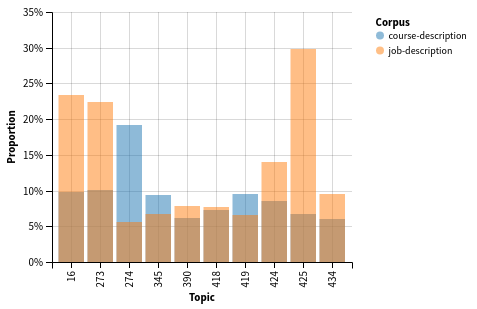
\includegraphics[width=0.5\textwidth]{figs/strict-overlap}
  \caption{Strictly overlapping topics for $\rho=0.02$ and $\theta=0.055$}~\label{fig:overlap}
\end{figure}


\section{Discussion}

Perhaps the most striking result is that only ten topics of five hundred total can be considered strictly overlapping.
That is, there is only two percent overlap.
An additional twenty four topics (for a total of thirty four) can be considered ``weakly overlapping'' by relaxing the $\theta$ constraint to only one $D_j$ rather than all.
However, this still only gives a Jaccard similarity coefficient of 0.68.
There are several ways to interpret this.

The most direct reading of the data indicates, simply, that universities are not teaching to what the workforce expects.
Of the five hundred extracted topics, some are expressed by curricular data, some are expressed by career data, but the degree of overlap is low.
The low Jaccard index of the two sets indicates a fairly significant dissimilarity.

However, perhaps the most probable interpretation is that the number of extracted topics was simply significantly too low.
Considering that almost fifty thousand documents were modeled across the two corpora, and considering that any given document can express many different topics, five hundred topics is simplty too low a number.
Increasing that count to several hundred thousand would most likely garner significantly higher levels of overlap.
The LDA process is storage and memory bound.
Increasing the number of topics significantly beyond five hundred would require significant computational resources.

One future extension to this work is the systematic analysis of the hyper parameters.
Specifically: the number of inferred topics ($k$), relevance ($\rho$), and intersection ($\theta$).
The author hypothesizes that an optimal maximum Jaccard index can be obtained most directly by increasing $k$ beyond five hundred.


\section{Acknowledgments}
The author would like to thank Eric Ianni of Georgia Tech for his feedback
and critiques.


\balance{}

\bibliographystyle{sigchi}
\bibliography{references}

\end{document}
